\chapter{Theory and Motivation}
\paragraph{} This chapter further describes the setting of our work and gives the reader some overview of the tools and techniques we used in our work. Section~\ref{sec:gantheory} first provides the theoretical background necessary to better understand the setting in which our work take place. Then, section~\ref{sec:doominfo} describes and motivates the choice of the game we work with. 

\section{Theoretical Background}
\label{sec:gantheory}
\subsection{Overview}
\paragraph{} As the main model for generating levels we selected the Generative Adversarial Networks. This model showed good results in many applications and it's increasingly more adopted and studied in the research community. Due to this, a large variety of different architectures and variants are designed in order to improve the original model. In this section we present an introduction to the \gls{gan} model and the main variant we considered for selecting the final model. 

\subsubsection{GAN}
\label{sec:introgan}
\paragraph{} Generative Adversarial Network, proposed by \citeauthor{gan} in \citetitle{gan} (\citeyear{gan}) \cite{gan}, are a model that gained gained increasingly more interest in the latest years. The main idea of this kind of generative model is to use two neural networks which are posed in an adversarial setting that models a two-player Minimax Game \cite[p.~276]{minimax}. In particular, a generative network $G$ is trained to capture the data distribution while a discriminator network $D$ estimates the probability that each sample comes from the real data distribution rather than the one generated by $G$. 
Equation \ref{eq:ganloss} shows the losses for D and G in the original \gls{gan} architecture\cite{gan}:

\begin{equation}
\label{eq:ganloss}
%\tag{WGAN-GP Critic Loss}
\begin{split}
L_{D}^{(i)} \gets & \frac{1}{m} \sum_{i=1}^m \left[
\log D\left({x}^{(i)}\right)
+ \log \left(1-D\left(G\left({z}^{(i)}\right)\right)\right)
\right] \\
%\tag{WGAN-GP Generator Loss}
L_{G}^{(i)} \gets & \frac{1}{m} \sum_{i=1}^m
\log \left(1-D\left(G\left({z}^{(i)}\right)\right)\right)
\end{split}
\end{equation}

where ${z}^{(i)}$ is a batch of random noise samples and ${x}^{(i)}$ is a batch of true data samples. \\*
The two networks are trained alternately by \textit{Backpropagation}, in this way the generator network can learn to produce better samples by using the discriminator output as a sort of feedback. 

\subsection{Deep Convolutional GAN (DCGAN)}
Typically, training a Generative Neural Network is a difficult task. This is, among other reasons, due to the need of balancing the generator and the discriminator during the minimax optimization. In order to overcome these difficulties, \citeauthor{gan:dcgan} proposed the DCGAN model \cite{gan:dcgan} which offer some improvements over the standard \gls{gan} architecture. The main modifications introduced are the use of convolutional layers instead of fully connected and max-pooling, the use of batch normalization \cite{batchnorm} and ReLu activation functions \cite{relu}. DCGAN architecture became one of the main baselines to build projects involving \glspl{gan} and compare new architectures. In our work we used the DCGAN layer structure showed in figure \ref{fig:dcganlayers} as a starting point for our experiments, which differs from ours for the presence of the conditioning input, the stride and the input size. These details on our architecture will be explained in chapter~\ref{ch:experiment}.

\begin{figure}[h!]
	\begin{center}
		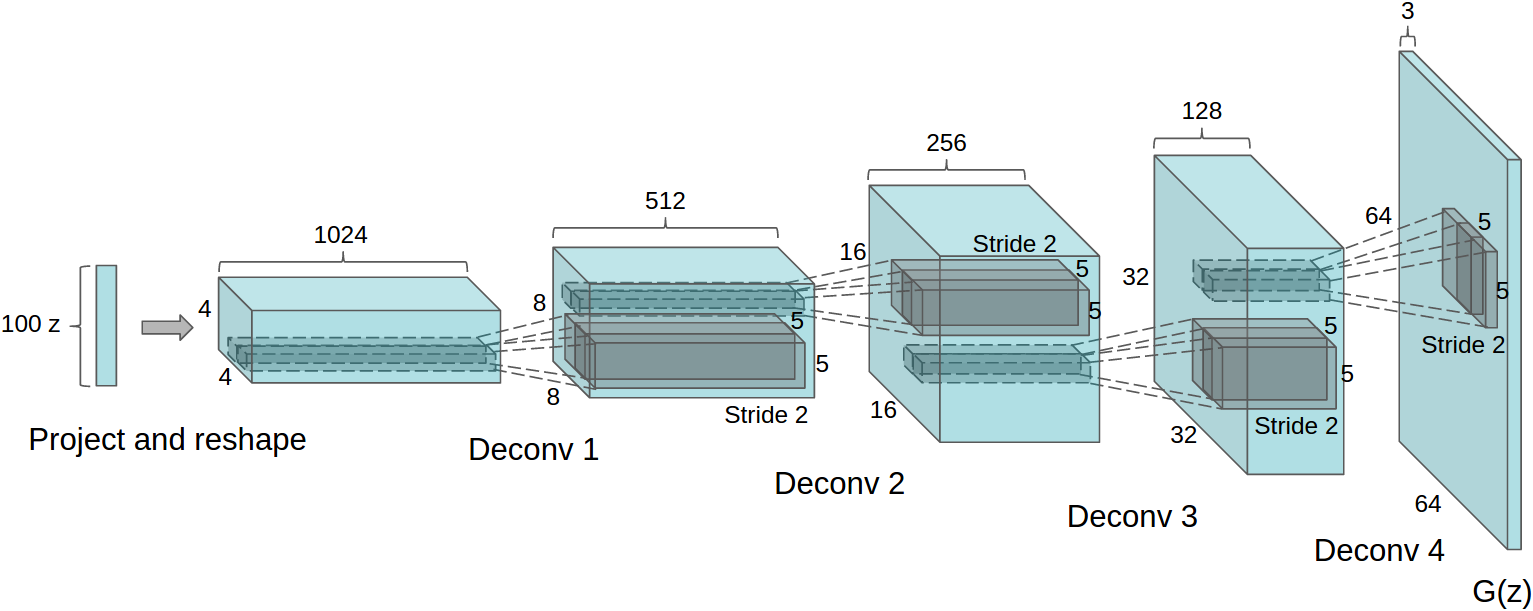
\includegraphics[width=1\linewidth]{DCGAN_layers}
	\end{center}
	
	\captionsetup{width=1\linewidth}
	\caption[Layers  from DCGAN, \citeauthor{gan:dcgan}]{DCGAN generator layers from the work of \citeauthor{gan:dcgan} on the LSUN dataset \cite[p.4]{gan:dcgan}.}
	\label{fig:dcganlayers}
	\medskip
\end{figure}

\subsection{Wasserstein GAN}
\paragraph{} Despite of the improvements, \glspl{gan} are still affected by some problems: training stability is dependent on the network structure, the training loss does not converge and not reflecting the actual sample quality. The Wasserstein GAN architecture, introduced by \citeauthor{wgan} \cite{wgan}, aims to mitigate these problems. The authors build a new loss function, based on the fact that training a GAN can be interpreted as minimizing the \textit{Jensen-Shannon divergence}\cite{jsdivergence}. They also prove how the Wasserstein (or Earth-Mover) \cite[\S~3]{wgan} distance is more sensible in the considered setting. \\* The resulting loss function is an approximation to the Wasserstein distance:

\begin{equation}
\label{eq:wganloss}
\begin{split}
L_{Critic}^{(i)} \gets & \mathbb{E}(D(X_{Gen})) - \mathbb{E}(D(X_{True}))\\
L_{Gen}^{(i)} \gets & -D(X_{Gen}) 
\end{split}
\end{equation}

This approximation is derived from an alternative formulation of the Wasserstein distance, which requires to calculate a supremum over \textit{K-Lipschitz} functions. To force the network to only model K-Lipschitz functions the weights of the critic network are clamped, and no output functions are applied to the discriminator function, in this case called \textit{critic}.  

\subsection{Wasserstein GAN with Gradient Penalty}
\label{sec:wgangp}
\paragraph{} \citeauthor{wgangp} remark in \cite{wgangp} that the WGAN architecture suffers from some optimization problems related to the weight clipping. Their experiment shows that gradient often vanishes or explodes if the weight clipping is not tuned carefully, and that this technique also biases the network toward too simple functions. To overcome these problems, they propose an alternative way to enforce the \textit{Lipschitz constraint} by keeping the gradient at unitary size. This involves adding a penalty term to the critic loss to enforce the constraint only along straight lines between the real and the generated data distribution, which leads to good results and performances.

\begin{equation}
\label{eq:gp}
\begin{split}
\hat{X} & \gets \epsilon X_{True} + (1-\epsilon) X_{Gen} \\
G_p & \gets (\| \nabla_{\hat{X}}D(\hat{X}) \|_2 - 1 )^2
\end{split}
\end{equation}

Results obtained from \citeauthor{wgangp} on the LSUN dataset are shown in Figure \ref{fig:wgangp}.
\begin{figure}[h!]
	\begin{center}
		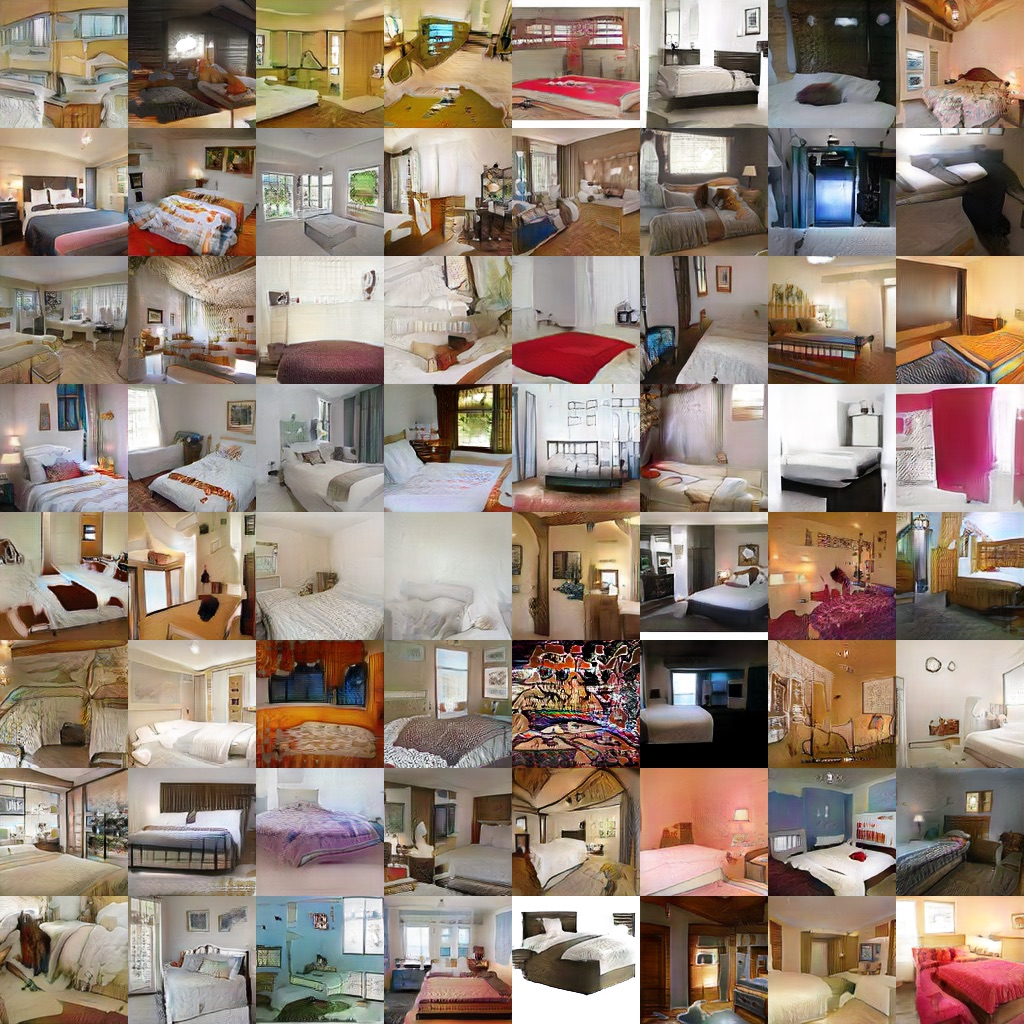
\includegraphics[width=1\linewidth]{wgangp_example}
	\end{center}
	
	\captionsetup{width=1\linewidth}
	\caption[Samples from WGAN-GP, \citeauthor{wgangp}]{Examples from the work of \citeauthor{wgangp} on the LSUN dataset using WGAN-GP. \cite[p.8]{wgangp}}
	\label{fig:wgangp}
	\medskip
\end{figure}

\subsubsection{Conditional GAN}
\paragraph{} In our work we apply a modification of the \gls{gan} model introduced by \citeauthor{conditionalgan} \cite{conditionalgan} to the WGAN-GP, which allows to condition the data generation to class labels. The motivation we chose this model is to allow with some extent the generation process, instead of generating random samples; this also allows the network learn useful information encoded in the feature vector and exploit it to generate better results. The logical structure of the adopted generative model is summarized in section \ref{sec:modelstructure}.


\subsubsection{Additional Architectures}
\paragraph{} Due to the novelty of this model, many researches have been conducted to improve the quality performances of \glspl{gan}, leading to a variety of proposed new architectures. They can be classified as modifications to the underlying neural network architectures or even to the conceptual setting of the model itself, by means of changes to the loss function or the training algorithm. Other, less formal but still effective adjustment to the proposed models are the so called "tricks" in machine learning discussion communities, which adoption is often suggested in order to improve the difficult training of the network. The final architecture adopted is described in section \ref{sec:networkarch}.


\section{Game of choice: DOOM}
\label{sec:doominfo}
\subsection{Description}
\paragraph{} DOOM is a video-game produced \textit{Id Software} in 1993, and can be considered one of the games that defined the First Person Shooter genre. Gameplay consisted in traversing a series of levels populated by several enemies, and the player had the possibility to collect weapons, ammunition and power-ups in order to reach the exit of the level. Often, in order to reach the exit point, the player had to explore the level in order to find some keys required to open the doors that blocked the path. DOOM levels are divided in episodes of 8\/9 levels each. The first episode was released as shareware and \textit{Id Software} greatly encouraged the diffusion of the game. This contributed to the large celebrity the game had in a time in which internet was still not accessible to anyone.

\subsection{Motivation}

\paragraph{} The domain we chose for this work is that of First Person Shooter levels, which usually require the player a more explorative approach as opposed to platform games that are typically traversed in a single direction. This different type of exploration usually requires an higher dimensional representation of the levels, which makes working with fps levels more difficult. One of the peculiarities of this game engine is that the levels actually develop on a 2d plane, with the height added separately. In other words, rooms cannot overlap on the height dimension, and often game designers succeeded in producing this type of illusion. This makes DOOM a good game for researching on first person shooters levels while keeping a simple 2d representation. 

\paragraph{} Another important feature of the Doom Game Engine is that it provided native "mods" support. This fact encouraged many people to develop and exchange their levels for DOOM, and soon this produced a large level database of levels which is still expanding nowadays. Thanks to a large active community it is possible to easily find many resources and specifications to work with DOOM levels and understand how the game engine works.

\section{Summary}
In this chapter we described some of the main Generative Adversarial Network architectures that are currently available in the literature, starting from the standard GAN to the most used improvements. Then, we briefly described the motivation we selected DOOM as the game to work with. In the next chapter we give a more in-depth explanation of how the Doom Engine works and levels are described, while in chapter \ref{ch:system_design} we give a logical description of how we implemented the GAN architecture. 